

%!TEX TS-program = xelatex
%!TEX encoding = UTF-8 Unicode

\documentclass[a4paper,10pt]{extarticle}

%\usepackage{blindtext} % Package to generate dummy text throughout this template 


%\usepackage[sc]{mathpazo} % Use the Palatino font
\usepackage[T1]{fontenc} % Use 8-bit encoding that has 256 glyphs
\linespread{1}
\usepackage{microtype} % Slightly tweak font spacing for aesthetics

\usepackage[english,russian]{babel} 
\usepackage{fontspec} 
\defaultfontfeatures{Ligatures={TeX},Renderer=Basic} 
\setmainfont[Ligatures={TeX,Historic}]{Times New Roman} 

% Language hyphenation and typographical rules

\sloppy             % Избавляемся от переполнений
\hyphenpenalty=1000 % Частота переносов
\clubpenalty=10000  % Запрещаем разрыв страницы после первой строки абзаца
\widowpenalty=10000 % Запрещаем разрыв страницы после последней строки абзаца

\usepackage{textcase}    % to connect the registers 

\usepackage{indentfirst}   %следующая после заголовка раздела строка текста как была, так и осталась лишённой отступа. Так принято в британской полиграфической традиции

\usepackage{geometry}
\geometry{left=2.5cm}
\geometry{right=2cm}
\geometry{top=2cm}
\geometry{bottom=2.5cm}

%\usepackage[hmarginratio=1:1,top=32mm,columnsep=20pt]{geometry} % Document margins
\usepackage[hang, small,labelfont=bf,up,textfont=it,up]{caption} % Custom captions under/above floats in tables or figures
\usepackage{booktabs} % Horizontal rules in tables

%\usepackage{lettrine} % The lettrine is the first enlarged letter at the beginning of the text

\usepackage{enumitem} % Customized lists
\setlist[itemize]{noitemsep} % Make itemize lists more compact

\usepackage{abstract} % Allows abstract customization
\renewcommand{\abstractnamefont}{\normalfont\bfseries} % Set the "Abstract" text to bold
%\renewcommand{\abstracttextfont}{\normalfont\small\itshape} % Set the abstract itself to small italic text

\renewcommand{\baselinestretch}{1}
\parindent 5ex


\usepackage{titlesec} % Allows customization of titles
\renewcommand\thesection{\Roman{section}} % Roman numerals for the sections
\renewcommand\thesubsection{\roman{subsection}} % roman numerals for subsections
\titleformat{\section}[block]{\large\centering\bfseries\MakeTextUppercase}{\thesection.}{1em}{} % Change the look of the section titles
\titleformat{\subsection}[block]{\large}{\thesubsection.}{1em}{} % Change the look of the section titles

\usepackage{fancyhdr} % Headers and footers
\pagestyle{fancy} % All pages have headers and footers
\fancyhead{} % Blank out the default header
\fancyfoot{} % Blank out the default footer
\fancyhead[C]{Ефименко А.Д. $\bullet$ Май 20120 $\bullet$ МГЭМ им. А.Д. Сахарова БГУ} % Custom header text
\fancyfoot[RO,LE]{\thepage} % Custom footer text

\usepackage{titling} % Customizing the title section

\usepackage{hyperref} % For hyperlinks in the PDF


\RequirePackage{caption}
\DeclareCaptionLabelSeparator{defffis}{ -- } % Разделитель
\captionsetup[figure]{justification=centering, labelsep=defffis, format=plain} % Подпись рисунка по центру
\captionsetup[table]{justification=raggedright, labelsep=defffis, format=plain, singlelinecheck=false} % Подпись таблицы слева
\addto\captionsrussian{\renewcommand{\figurename}{Рис.}} % Имя фигуры

% Пути к каталогам с изображениями
\usepackage{graphicx} % Вставка картинок и дополнений
\DeclareGraphicsExtensions{.png,.jpg}
\graphicspath{{image/}} 					%{image/userguide/}

\newcommand{\addimg}[4]{ % Добавление одного рисунка
    \begin{figure}
        \centering
        \includegraphics[width=#2\linewidth]{#1}
        \caption{#3} \label{#4}
    \end{figure}
}
\newcommand{\addimghere}[4]{ % Добавить рисунок непосредственно в это место
    \begin{figure}[H]
        \centering
        \includegraphics[width=#2\linewidth]{#1}
        \caption{#3} \label{#4}
    \end{figure}
}



%----------------------------------------------------------------------------------------
%	TITLE SECTION
%----------------------------------------------------------------------------------------

\setlength{\droptitle}{-6\baselineskip} % Move the title up

\pretitle{\begin{center}\bfseries\MakeTextUppercase}
%\hyphenation
 % Article title formatting \bfseries -- жирный шрифт \itshape -- курсив
\posttitle{\end{center}} % Article title closing formatting
\title{Рабочая сила медицинской физики мирового сообщества и ее 
сопоставление в Республике Беларусь} % Article title


\begin{author}
{
\textsc 
{\MakeTextUppercase{\bfseries \normalsize Workforce of medical physics of the world community}}\\{\MakeTextUppercase{\bfseries \normalsize and its comparison in the Republic of Belarus }} \\ \\{\bfseries А.Д. Ефименко, Л.А. Липницкий} \\ \\ {\bfseries A.D. Ephimenko, L.A. Lipnitsky}\\ \\% Your name    and its comparison in the Republic of Belarus
%\thanks{A thank you or further information} \\[1ex] 
\normalsize \itshape Белорусский государственный университет МГЭИ им. А.Д.Сахарова БГУ \\ 
\normalsize \itshape г. Минск Республика Беларусь \\ 
\normalsize \itshape ISEU BSU, Minsk Republic of Belarus \\ % Your institution
\normalsize \href{mailto:ialexefimenko@icloud.com}{ialexefimenko@icloud.com} % Your email address
}
\end{author}
%\date{\today} % Leave empty to omit a date
\renewcommand{\maketitlehookd}
{
\begin{abstract}
\noindent \normalsize \scshape Сегодня профессия медицинской физики является признанной, устоявшейся и зрелой, которая претерпевает значительный рост и изменения, причем многие из этих изменений обусловлены научными, техническими и медицинскими достижениями. В настоящее время рабочая сила медицинской физики достаточна для удовлетворения общественных потребностей в большинстве стран мира, Беларусь в этом только набирает обороты, но квалифицированного персонала с каждым годом становится больше, хотя и существуют явные проблемы в образовательном аспекте. Для становления квалифицированным (клиническим) медицинским физиком определен план обучения, и казалось, какие могут быть проблемы на этот счет. Но нет, имеются потенциальные проблемы по дефициту кадров, которые могут возникнуть в течение нескольких лет.  Некоторые из определяющих факторов хорошо известны, такие как увеличение числа раковых заболеваний, что приводит к увеличению рабочей нагрузки, в то время как другие, такие как будущее использование лучевых методов лечения и изменения в экономической политике здравоохранения, являются неопределенными и затрудняют прогнозирование будущего состояния рабочей силы в течение следующих нескольких лет. В работе рассматриваются некоторые из основных факторов, определяющих спрос и предложение медицинских физиков в мире, и в частности, Республике Беларусь. Описаны общие характеристики работников, включая информацию о ее численности и уровне образования. На основе анализа литературных данных были выдвинуты рекомендации по продвижению и развитию медицинских физиков в Беларуси, а также рассмотрены перспективы будущего персонала на основании существующих проблем в мировом сообществе. \\ \\
Today, the medical physics profession is recognized, established, and Mature, and is undergoing significant growth and changes, many of which are due to scientific, technical, and medical advances. Currently, the workforce of medical physics is sufficient to meet the public needs in most countries of the world, Belarus is only gaining momentum, but the number of qualified personnel is increasing every year, although there are obvious problems in the educational aspect. To become a qualified (clinical) medical physicist, a training plan was defined, and it seemed that there might be problems in this regard. But no, there are potential problems with staff shortages that may occur within a few years.  Some of the determinants are well known, such as an increase in the number of cancers that lead to increased workloads, while others, such as the future use of radiation treatments and changes in economic health policy, are uncertain and make it difficult to predict the future state of the workforce over the next few years. The paper considers some of the main factors that determine the demand and supply of medical physicists in the world, and in particular in the Republic of Belarus. General characteristics of employees are described, including information about their number and level of education. Based on the analysis of the literature data, recommendations were made for the promotion and development of medical physicists in Belarus, as well as the prospects for future personnel based on existing problems in the world community.
% \scshape -- отмена курсива 
 \\


\itshape Ключевые слова: \scshape 
 
\end{abstract}
}


%----------------------------------------------------------------------------------------

\begin{document}

% Print the title
\maketitle

%----------------------------------------------------------------------------------------
%	ARTICLE CONTENTS
%----------------------------------------------------------------------------------------

\section{Введение}{\parindent 1.27cm}

Почти сразу же после открытия рентгеновских лучей в конце XIX века \cite{W. C. Röntgen} ионизирующее излучение нашло применение в диагностике и лечении широкого спектра заболеваний человека, а также в промышленности, научных кругах, энергетике и национальной обороне. Несмотря на то, что мировое федеральное правительство содействовало созданию сообщества профессионалов, обеспечивающих безопасное и полезное использование радиации, число специалистов по радиации в последнее время тревожно сократилось,, когда в нашей стране еще происходит ее развитие,  о чем свидетельствуют документы нескольких уважаемых организаций \cite{USGAO 2014}\cite{HPS 2013}\cite{NCRP 2015}. Совсем недавно МКРЗ опубликовали заявление под названием <<Где находятся специалисты по радиации?>>, которая предупредила о возможности того, что будущие национальные потребности в ряде соответствующих секторов, включая медицину, могут остаться неудовлетворенными \cite{NCRP 2015}.

Подчеркивается большая неопределенность, сильная зависимость от предполагаемых входных параметров и высокий уровень сложности проблемы в подходе к профессии медицинский физик \cite{Mills MD.2014}. Кроме того, она продолжает существенно развиваться. Разумно рассмотреть возможность того, что трудовых ресурсов может быть недостаточно, и продумать стратегии мониторинга риска для мирового сообщества медицинских физиков.

Касательно Беларуси, профессия еще неустоявшаяся. Выходя на мировой уровень, в первую очередь необходимо разработать и внедрить приспособления и технологии для обеспечения качества диагностических и терапевтических процедур. организовать работу по разъяснению работникам организации здравоохранения вопросов обеспечения безопасности пациентов и работников, после этого и решение задач будет обсуждаться совместно с международным сообществом.


\addimg{edpath}{1}{Пути обучения в области медицинской физики \cite{Silverstein}.}{edpath}
%\lettrine[nindent=0em,lines=3]{L} orem ipsum dolor sit amet, consectetur adipiscing elit.
%\blindtext % Dummy text

%\blindtext % Dummy text

%------------------------------------------------

\section{Кадровая характеристика медицинской физики}

В мире насчитывается около 24 000 медицинских физиков \cite{IOMP}, из которых чуть более трети, или 8205, находятся в Соединенных Штатах \cite{AAPM1} и 2303 -- в Европе \cite{Lievens}. Дополнительная и более конкретная информация поступает от Американской ассоциации физиков в медицине (AAPM), которая ежегодно проводит опрос своих членов и предоставляет описательные статистические данные, имеющие отношение к национальной рабочей силе, но только на пространстве США. К примеру, у них на 2018 год, по данным 2565 респондентов, 51\% и 49\% имели степень магистра и доктора наук соответственно. Большинство (76\%)  медицинских физиков занимались радиационной онкологией в качестве своей основной специальности, и почти все (94\%) были заняты на полный рабочий день, и только 3\% были фрилансеры-консультанты. Как видно, проблем с численностью медицинской рабочей силы нет, в целом она находится в равновесии с потребностями страны. В США и нескольких других странах медицинская физика четко определенная, устоявшаяся и зрелая профессия. 

В СССР медицинская физика появилась в 60--e годы прошлого века, на данный момент в России насчитывается около 500 человек при очень низкой <<плотности>> населения \cite{Костылёв}, а в нашей стране и вовсе на 468 человек меньше \cite{Тарутин}. ..............




%------------------------------------------------

\section{Высшее образование и профессиональная подготовка}
Профессия медицинская физика пользовалась успехом на протяжении многих десятилетий, в результате возникшего интеллектуального разнообразия подхода обучения -- для многих физиков до начала нынешнего века их образование было докторской степенью по физике вместе с обучением на рабочем месте и самоподготовкой по медицинской физике.  Однако, компетентность и готовность медицинских физиков к выполнению клинической работы были весьма сомнительны. 

Сегодня пути к тому, чтобы стать квалифицированным (клиническим) медицинским физиком, четко определены и стандартизированы согласно рекомендациям МКРЗ. Рис.\ref{edpath} показывает траектории обучения, начинающиеся с получения степени бакалавра по физике (или равнозначимой смежной области) и заканчивающиеся получением начального уровня в данной специальности.
Согласно AAPM, квалифицированный медицинский физик сможет получить степень магистра и/или доктора в области физики, медицинской физики, биофизики, радиологической физики, медицинской физики здоровья или равнозначимых дисциплин в аккредитованном колледже/университете. Кроме того, квалификация требует сертификации в конкретной области медицинской физики, соответствующим национальным органом по сертификации и соблюдения текущих требований к непрерывному образованию \cite{AAPM 2016b}. 

Так устроено образование за рубежом. В РБ с образованием ситуация такова: Минский государственный экологический институт имени Андрея Дмитриевича Сахарова при Белорусском государственном университете выпускает с 2018 года студентов по специальности <<медицинский физик>>. Затем следует поступление на магистратуру, после чего -- заступление на рабочее место по обслуживанию ускорителей, по разработке и внедрению приспособлений технологий для обеспечения качества диагностических и терапевтических процедур, занимается организаторской работой по разъяснению работникам организации здравоохранения вопросов обеспечения безопасности пациентов и работников. ..............

%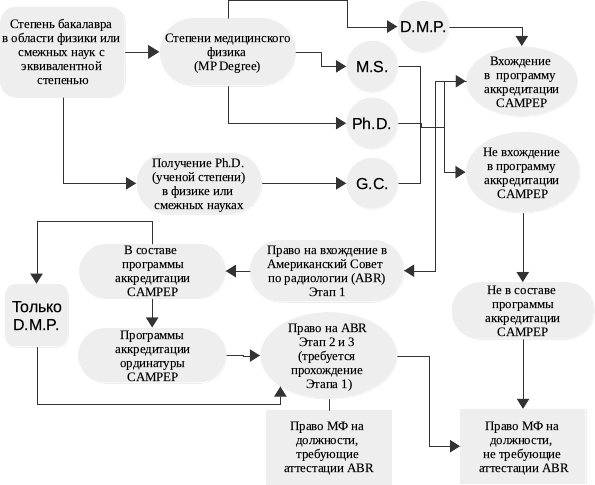
\includegraphics{edpath} \\ {Рис.1 -- }{Внутренние и внешние связи подсистемы управления услугами}




%\begin{table}
%\caption{Пример таблицы}
%\centering
%\begin{tabular}{llr}
%\toprule
%\multicolumn{2}{c}{Name} \\
%\cmidrule(r){1-2}
%First name & Last Name & Grade \\
%\midrule
%John & Doe & $7.5$ \\
%Richard & Miles & $2$ \\
%\bottomrule
%\end{tabular}
%\end{table}

%\blindtext % Dummy text
%
%\begin{equation}
%\label{eq:emc}
%\frac{dp}{dt}=\vec{F}
%\end{equation}

%\blindtext % Dummy text

%------------------------------------------------

\section{Профессиональные аспекты релятивности работников}



%\subsection{}



%A statement requiring citation \cite{No174}.
%\blindtext % Dummy text

%\subsection{}

%\blindtext % Dummy text
%------------------------------------------------

\section{Заключение}

%------------------------------------------------

%\section{Рекомендации по продвижению соответствующих специалистов}
%----------------------------------------------------------------------------------------
%	REFERENCE LIST
%----------------------------------------------------------------------------------------

\begin{thebibliography}{99} % Bibliography - this is intentionally simple in this template

\bibitem {W. C. Röntgen}
W. C. Röntgen. Ueber eine neue Art von Strahlen // Sonderabbdruck aus den Sitzungsberichten der Würzburger Physik.medic. Gesellschaft. — 1895;

\bibitem {Silverstein}
Silverstein E, Burmeister J, Fullerton G. SDAMPP student guide to a medical physics career. Alexandria, VA: Society of Directors of Academic Medical Physics Programs; 2016;

\bibitem {USGAO 2014}
U.S. Government Accountability Office. Federal workforce: recent trends in federal civilian employment and compensation. Washington, DC: GAO;14 -- 215; 2014;

\bibitem {HPS 2013}
Health Physics Society. Health physics education reference book. Health Physics Society Academic Education Committee. McLean, VA: HPS; 2010;

\bibitem {NCRP 2015}
National Council on Radiation Protection and Measurements. Where are the radiation professionals (WARP)? Bethesda, MD: NCRP; Statement No. 12; 2015;

\bibitem {Mills MD.2014} 
Mills MD. The meaning of the MS degree in medical physics, part 3. 2014;

\bibitem {IOMP}
International Organization for Medical Physics. Organization. Athens, Greece: IOMP; 2016. Available at www.iomp.org/? q=content/organisation. Accessed 9 August 2016;

\bibitem {AAPM1}
American Association of Physicists in Medicine. Professional survey report, calendar year 2015. College Park, MD: AAPM; 2016a;

\bibitem {Lievens}
Lievens Y, Defourny N, Coffey M, Borras JM, Dunscombe P, Slotman B, Malicki J, Bogusz M, Gasparotto C, Grau C, Kokobobo A, Sedlmayer F, Slobina E, Coucke P, Gabrovski R, Vosmik M, Eriksen JG, Jaal J, Dejean C, Polgar C, Johannsson J, Cunningham M, Atkocius V, Back C, Pirotta M, Karadjinovic V, Levernes S, Maciejewski B, Trigo ML, Šegedin B, Palacios A, Pastoors B, Beardmore C, Erridge S, Smyth G, Soler RC. Radiotherapy staffing in the European countries: final results from the ESTRO-HERO survey. Radiother Oncol 112:178–186; 2014.


\bibitem {Костылёв}
Костылёв, В.А., Наркевич, Б.Я.. Радиационная медицинская физика: прошлое, настоящее и будущее. Медицинская радиология и радиационная безопасность. -- 2006, --  Том 51, N1;

\bibitem {Тарутин}
Патыко, Д.. Нужны ли в больницах медицинские физики? -- Медицинский вестник. -- 2019. -- N 39 от 3 октября. -- с. 4;

\bibitem {AAPM 2016b}
American Association of Physicists in Medicine. Medical physicist. Definition of a qualified medical physicist. 2016b. Available at \href{https://w3.aapm.org/medical_physicist/fields.php}{Definition of a Qualified Medical Physicist}. Accessed 9 August 2016;


 
%\bibitem {No174}
%Guibelade E., Christifides S., Caruna C.J., Evans S., van der Putten W.
%\newblock Radiation Protection 174. European Guidelines on medical physics expert.  
%\newblock Directorate-General for Energy Directorate D — Nuclear Safety. Fuel Cycle Unit D.3 — Radiation Protection.
%2014;	%	{\em Human Nature}

%\bibitem [3]
\end{thebibliography}

%----------------------------------------------------------------------------------------

\end{document}
